\documentclass{ximera}

\usepackage{epsfig}

\graphicspath{
  {./}
  {figures/}
}


\usepackage{morewrites}

%\newcounter{ccounter}
%\setcounter{ccounter}{1}
%\newcommand{\Chapter}[1]{\setcounter{chapter}{\arabic{ccounter}}\chapter{#1}\addtocounter{ccounter}{1}}

%\newcommand{\section}[1]{\section{#1}\setcounter{thm}{0}\setcounter{equation}{0}}

%\renewcommand{\theequation}{\arabic{chapter}.\arabic{section}.\arabic{equation}}
%\renewcommand{\thefigure}{\arabic{chapter}.\arabic{figure}}
%\renewcommand{\thetable}{\arabic{chapter}.\arabic{table}}

%\newcommand{\Sec}[2]{\section{#1}\markright{\arabic{ccounter}.\arabic{section}.#2}\setcounter{equation}{0}\setcounter{thm}{0}\setcounter{figure}{0}}

\newcommand{\Sec}[2]{\section{#1}}

\setcounter{secnumdepth}{2}
%\setcounter{secnumdepth}{1} 

%\newcounter{THM}
%\renewcommand{\theTHM}{\arabic{chapter}.\arabic{section}}

\newcommand{\trademark}{{R\!\!\!\!\!\bigcirc}}
%\newtheorem{exercise}{}

\newcommand{\dfield}{{\sf dfield9}}
\newcommand{\pplane}{{\sf pplane9}}

\newcommand{\EXER}{\section*{Exercises}}%\vspace*{0.2in}\hrule\small\setcounter{exercise}{0}}
\newcommand{\CEXER}{}%\vspace{0.08in}\begin{center}Computer Exercises\end{center}}
\newcommand{\TEXER}{} %\vspace{0.08in}\begin{center}Hand Exercises\end{center}}
\newcommand{\AEXER}{} %\vspace{0.08in}\begin{center}Hand Exercises\end{center}}

% BADBAD: \newcommand{\Bbb}{\bf}

\newcommand{\R}{\mbox{$\Bbb{R}$}}
\newcommand{\C}{\mbox{$\Bbb{C}$}}
\newcommand{\Z}{\mbox{$\Bbb{Z}$}}
\newcommand{\N}{\mbox{$\Bbb{N}$}}
\newcommand{\D}{\mbox{{\bf D}}}
\usepackage{amssymb}
%\newcommand{\qed}{\hfill\mbox{\raggedright$\square$} \vspace{1ex}}
%\newcommand{\proof}{\noindent {\bf Proof:} \hspace{0.1in}}

\newcommand{\setmin}{\;\mbox{--}\;}
\newcommand{\Matlab}{{M\small{AT\-LAB}} }
\newcommand{\Matlabp}{{M\small{AT\-LAB}}}
\newcommand{\computer}{\Matlab Instructions}
\newcommand{\half}{\mbox{$\frac{1}{2}$}}
\newcommand{\compose}{\raisebox{.15ex}{\mbox{{\scriptsize$\circ$}}}}
\newcommand{\AND}{\quad\mbox{and}\quad}
\newcommand{\vect}[2]{\left(\begin{array}{c} #1_1 \\ \vdots \\
 #1_{#2}\end{array}\right)}
\newcommand{\mattwo}[4]{\left(\begin{array}{rr} #1 & #2\\ #3
&#4\end{array}\right)}
\newcommand{\mattwoc}[4]{\left(\begin{array}{cc} #1 & #2\\ #3
&#4\end{array}\right)}
\newcommand{\vectwo}[2]{\left(\begin{array}{r} #1 \\ #2\end{array}\right)}
\newcommand{\vectwoc}[2]{\left(\begin{array}{c} #1 \\ #2\end{array}\right)}



\newcommand{\inv}{^{-1}}
\newcommand{\CC}{{\cal C}}
\newcommand{\CCone}{\CC^1}
\newcommand{\Span}{{\rm span}}
\newcommand{\rank}{{\rm rank}}
\newcommand{\trace}{{\rm tr}}
\newcommand{\RE}{{\rm Re}}
\newcommand{\IM}{{\rm Im}}
\newcommand{\nulls}{{\rm null\;space}}

\newcommand{\dps}{\displaystyle}
\newcommand{\arraystart}{\renewcommand{\arraystretch}{1.8}}
\newcommand{\arrayfinish}{\renewcommand{\arraystretch}{1.2}}
\newcommand{\Start}[1]{\vspace{0.08in}\noindent {\bf Section~\ref{#1}}}
\newcommand{\exer}[1]{\noindent {\bf \ref{#1}}}
\newcommand{\ans}{}
\newcommand{\matthree}[9]{\left(\begin{array}{rrr} #1 & #2 & #3 \\ #4 & #5 & #6
\\ #7 & #8 & #9\end{array}\right)}
\newcommand{\cvectwo}[2]{\left(\begin{array}{c} #1 \\ #2\end{array}\right)}
\newcommand{\cmatthree}[9]{\left(\begin{array}{ccc} #1 & #2 & #3 \\ #4 & #5 &
#6 \\ #7 & #8 & #9\end{array}\right)}
\newcommand{\vecthree}[3]{\left(\begin{array}{r} #1 \\ #2 \\
#3\end{array}\right)}
\newcommand{\cvecthree}[3]{\left(\begin{array}{c} #1 \\ #2 \\
#3\end{array}\right)}
\newcommand{\cmattwo}[4]{\left(\begin{array}{cc} #1 & #2\\ #3
&#4\end{array}\right)}

\newcommand{\Matrix}[1]{\ensuremath{\left(\begin{array}{rrrrrrrrrrrrrrrrrr} #1 \end{array}\right)}}

\newcommand{\Matrixc}[1]{\ensuremath{\left(\begin{array}{cccccccccccc} #1 \end{array}\right)}}



\renewcommand{\labelenumi}{\theenumi)}
\newenvironment{enumeratea}%
{\begingroup
 \renewcommand{\theenumi}{\alph{enumi}}
 \renewcommand{\labelenumi}{(\theenumi)}
 \begin{enumerate}}
 {\end{enumerate}\endgroup}



\newcounter{help}
\renewcommand{\thehelp}{\thesection.\arabic{equation}}

%\newenvironment{equation*}%
%{\renewcommand\endequation{\eqno (\theequation)* $$}%
%   \begin{equation}}%
%   {\end{equation}\renewcommand\endequation{\eqno \@eqnnum
%$$\global\@ignoretrue}}

%\input{psfig.tex}

\author{Martin Golubitsky and Michael Dellnitz}

%\newenvironment{matlabEquation}%
%{\renewcommand\endequation{\eqno (\theequation*) $$}%
%   \begin{equation}}%
%   {\end{equation}\renewcommand\endequation{\eqno \@eqnnum
% $$\global\@ignoretrue}}

\newcommand{\soln}{\textbf{Solution:} }
\newcommand{\exercap}[1]{\centerline{Figure~\ref{#1}}}
\newcommand{\exercaptwo}[1]{\centerline{Figure~\ref{#1}a\hspace{2.1in}
Figure~\ref{#1}b}}
\newcommand{\exercapthree}[1]{\centerline{Figure~\ref{#1}a\hspace{1.2in}
Figure~\ref{#1}b\hspace{1.2in}Figure~\ref{#1}c}}
\newcommand{\para}{\hspace{0.4in}}

\renewenvironment{solution}{\suppress}{\endsuppress}

\ifxake
\newenvironment{matlabEquation}{\begin{equation}}{\end{equation}}
\else
\newenvironment{matlabEquation}%
{\let\oldtheequation\theequation\renewcommand{\theequation}{\oldtheequation*}\begin{equation}}%
  {\end{equation}\let\theequation\oldtheequation}
\fi

\makeatother


\title{mo12.tex}

\begin{document}
\begin{abstract}
BADBAD
\end{abstract}
\maketitle

\chapter{Bifurcation Theory}

\subsection*{Section~\protect{\ref{S:TSPM}} Two Species Population Models}
\rhead{S:TSPM}{TWO SPECIES POPULATION MODELS}

\exer{c9.1.5}
\ans Predators eat prey faster in the first system \Ref{E:prpr1} than in 
the second system \Ref{E:prpr2}.

\soln  In the predator prey system \Ref{e:PP}, the $x$ variable is the
prey population and the $y$ variable is the predator population.  The
question asks: In which system will the predator population cause a
larger decrease in the prey population.  That is, in which system is
the coefficient $\sigma_1$ in \Ref{e:PP} a larger negative number?  In
the first system $\sigma_1=-10$, while in the second system $\sigma_1=-0.1$.

\exer{c9.1.2}
\ans For $\mu = 6$, there is a center at $e_4 = (1,8)$.

\soln First compute the equilibria for general $\mu$ by solving
$\dot{x} = \dot{y} = 0$.  The equilibria of the system occur at
$e_1 = (0,0)$, $e_2 = (0,4)$, $e_3 = (-\frac{\mu}{2},0)$, and
$e_4 = (\frac{\mu}{2} - 2, 2\mu - 4)$.  A center occurs at an equilibrium
where the Jacobian has purely imaginary eigenvalues; that is, where
$\trace{(dJ)} = 0$ and $\det{(dJ)} > 0$.  The general Jacobian of this
system is
\[
(dJ)_{(x,y)} = \cmattwo{\mu + 4x - y}{-x}{y}{1 + x - 0.5y}.
\]
At the equilibria,
\[
(dJ)_{e_1} = \mattwo{\mu}{0}{0}{1}, \quad
(dJ)_{e_2} = \cmattwo{\mu - 4}{0}{4}{-1}, \quad
\]
\[
(dJ)_{e_3} = \cmattwo{-\mu}{\frac{\mu}{2}}{0}{1 - \frac{\mu}{2}}, \quad
(dJ)_{e_4} = \cmattwo{\mu - 4}{2 - \frac{\mu}{2}}{2\mu - 4}{1 -
\frac{\mu}{2}}.
\]
For each of these matrices, find $\mu$ such that $\trace{(dJ)} = 0$.  At
$e_1$, $e_2$, and $e_3$, when $\trace{(dJ)} = 0$, $\det{(dJ)} < 0$.
At $e_4$, solve $\trace(dJ) = 0$ to obtain $\mu = 6$.  Then $\det{(dJ)}
= 4 > 0$; so the point $(1,8)$ is a center when $\mu = 6$.

\newpage
\exer{c9.1.3}
Solve \Ref{e:PP} for $\dot{x} = \dot{y} = 0$ to find that there are
two equilibrium points, at $(0,0)$ and $(-\frac{\mu_2}{\sigma_2},
-\frac{\mu_1}{\sigma_1})$.  The second equilibrium is in the first
quadrant for any values of the constants that conform to the assumed
restrictions: $\mu_1 > 0$, $\mu_2 < 0$, $\sigma_1 < 0$, and
$\sigma_2 > 0$.  Load the system into {\tt pplane5} and graph with
several values for the constants to confirm that the nonzero
equilibrium is surrounded by periodic solutions.

\exer{c9.1.7}  Computer experiment.



\subsection*{Section~\protect{\ref{S:bifurcation}} Examples of Bifurcation}
\rhead{S:bifurcation}{EXAMPLES OF BIFURCATION}

\exer{c9.7.1}
\ans The bifurcation diagram (Figure~\ref{c9.7.1}) shows two equilibria
vanishing as $\rho$ increases through $0$.

\soln The equilibria of the equation occur when $0 = \frac{dx}{dt} =
\rho + x^2$; that is, when $\rho = -x^2$.  Thus, when $\rho < 0$, there
are two equilibria, at $x = \pm\sqrt{-\rho}$.  When $\rho = 0$, there is
one equilibrium at $x = 0$; and when $\rho > 0$, there are no real
equilibria.  Let $f(x,\rho) = \rho + x^2$.  If $\rho < 0$, 
then $f_x(\sqrt{-\rho},\rho) > 0$ and $f_x(-\sqrt{-\rho},\rho) < 0$. 
Thus, the equilibrium at $x = \sqrt{-\rho}$ is unstable, and the
equilibrium at $x = -\sqrt{-\rho}$ is stable.

\begin{figure}[htb]
                       \centerline{%
                       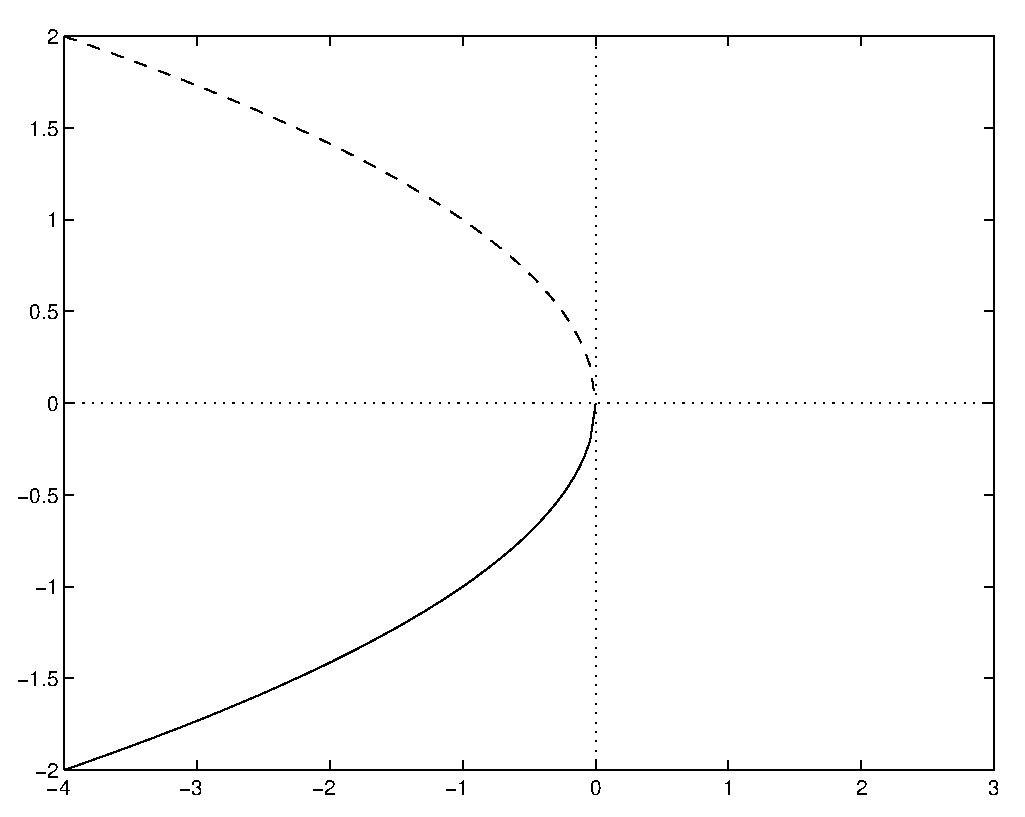
\psfig{file=exfigure/9-7-1.eps,width=3.0in}}
                \exercap{c9.7.1}
\end{figure}

\exer{c9.7.3}
\ans The maximum number of equilibria is 4.  This maximum occurs when
$8 < \rho < 13$.  The bifurcation diagram is shown in Figure~\ref{c9.7.3}.

\soln The equilibria of the equation occur when
$\rho = 3x^4 - 8x^3 - 6x^2 + 24x$.  Note that minimum and maximum points of
$\rho$ as a function of $x$ occur when $\rho_x = 0$.  Thus, minima occur
at $(x,\rho) = (-1,-19)$ and $(x,\rho) = (2,8)$, and a maximum occurs at
$(x,\rho) = (1,13)$.  So, as $\rho$ increases, two equilibria appear at
$\rho = -19$, two equilibria appear at $\rho = 8$, and two equilibria
disappear at $\rho = 13$.  When $x < -1$ and when $1 < x < 2$, equilibria
are stable.  For $-1 < x < 1$ and $2 < x$, equilibria are unstable.

\begin{figure}[htb]
                       \centerline{%
                       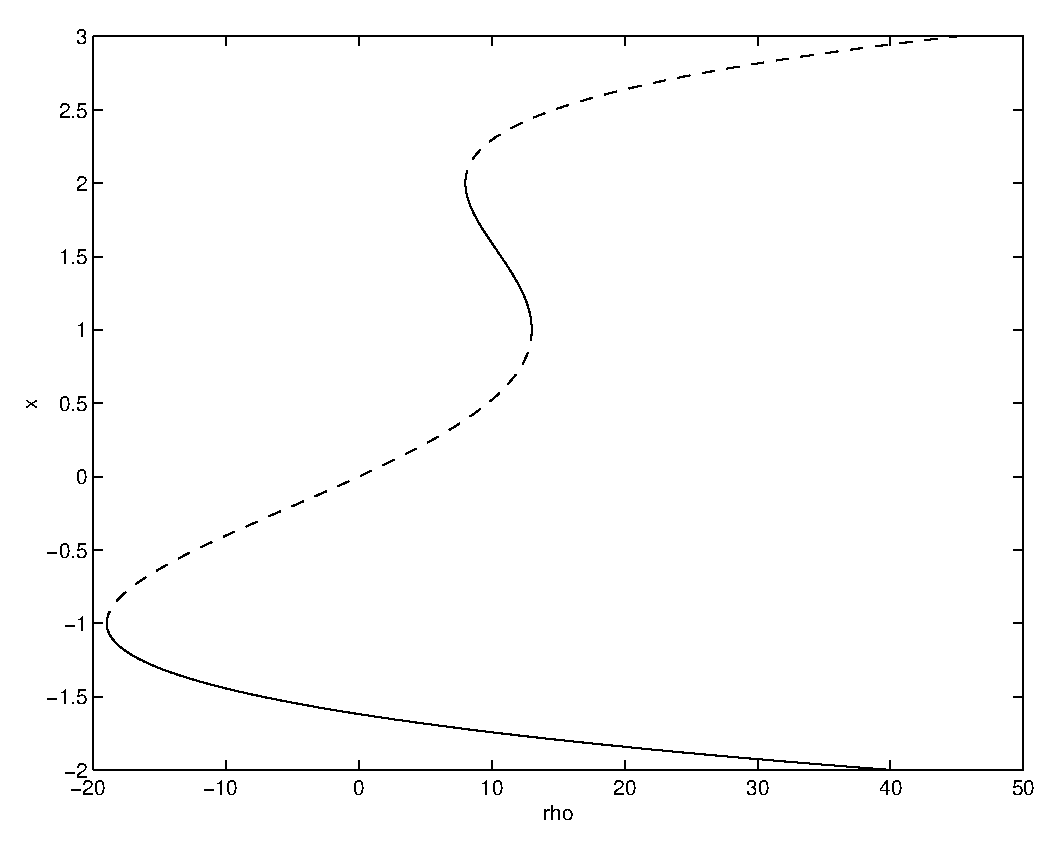
\psfig{file=exfigure/9-7-3.eps,width=3.0in}}
                \exercap{c9.7.3}
\end{figure}

\exer{c9.4.2}
\ans When $\rho = 0$, the differential equation can have a Hopf bifurcation 
only at $(x_0,y_0) = (2,1)$.

\soln A Hopf bifurcation can occur at an equilibrium point only when the 
trace of the Jacobian at this point is zero and the determinant of the 
Jacobian is positive.  In this case, the Jacobian of the differential 
equation at $\rho = 0$ is
\[
J_{(x,y)} = \mattwo{3 + 2x}{-4 - 4y}{14x - 3y}{-1 - 3x}.
\]
Then, $\trace(J_{(x,y)}) = 2 - x$; so $\trace(J) = 0$ when $x = 2$.  Solve
the differential equation for $\dot{x} = 0 = \dot{y}$ to find that $(x,y) =
(2,1)$ is an equilibrium point.  Since $\det(J_{(2,1)}) = 151 > 0$, this 
point can be a Hopf bifurcation point when $\rho = 0$.

\exer{e:uHopf}
The system is shown in Figure~\ref{e:uHopf}a with $\rho = -1$, and in
Figure~\ref{e:uHopf}b with $\rho = 1$.  In this system, a limit cycle
exists before the bifurcation point, whereas, in \Ref{E:Hopfbif}, the
limit cycle exists after the bifurcation point and vanishes at
$\rho = 0$.  Also, in this system, the limit cycle is unstable, while
the limit cycle of \Ref{E:Hopfbif} is stable.

\begin{figure}[htb]
                       \centerline{%
                       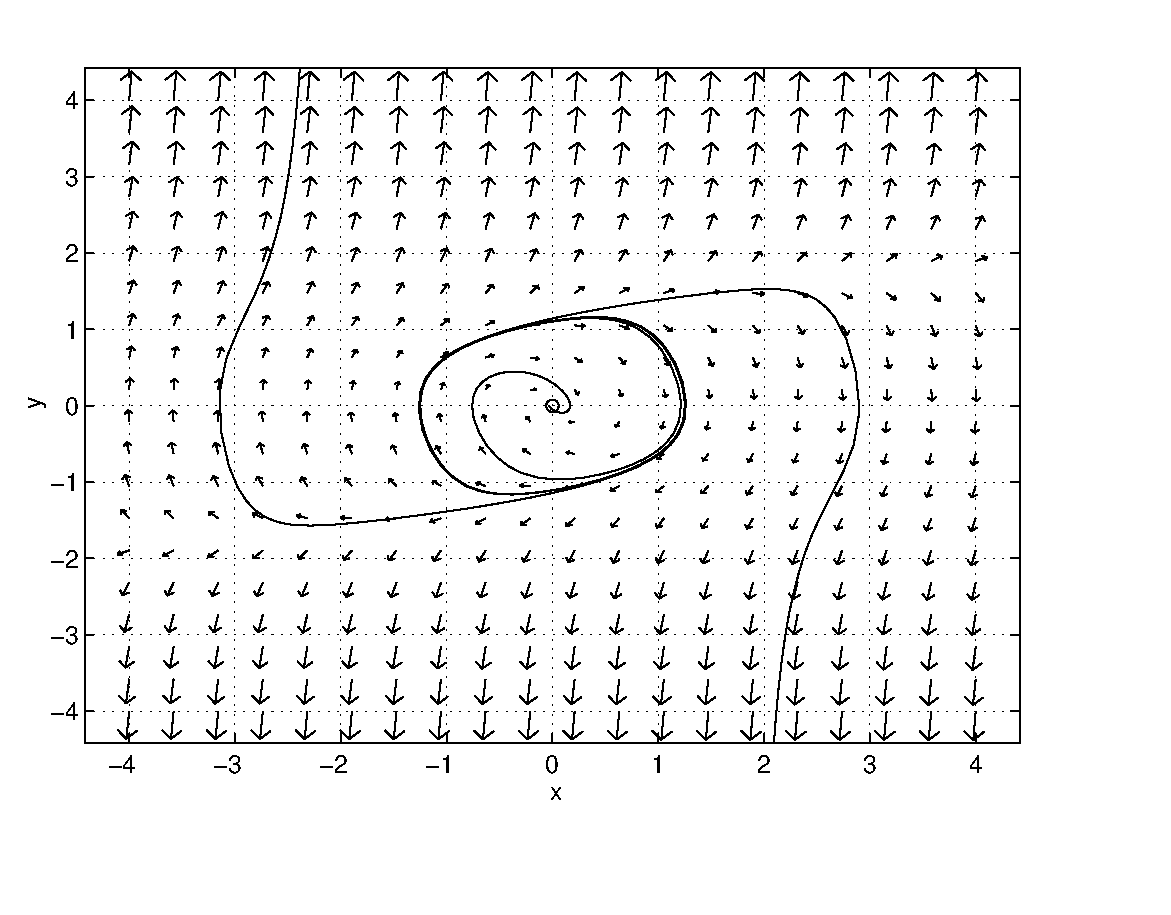
\psfig{file=exfigure/uHopfa.eps,width=2.75in}
                       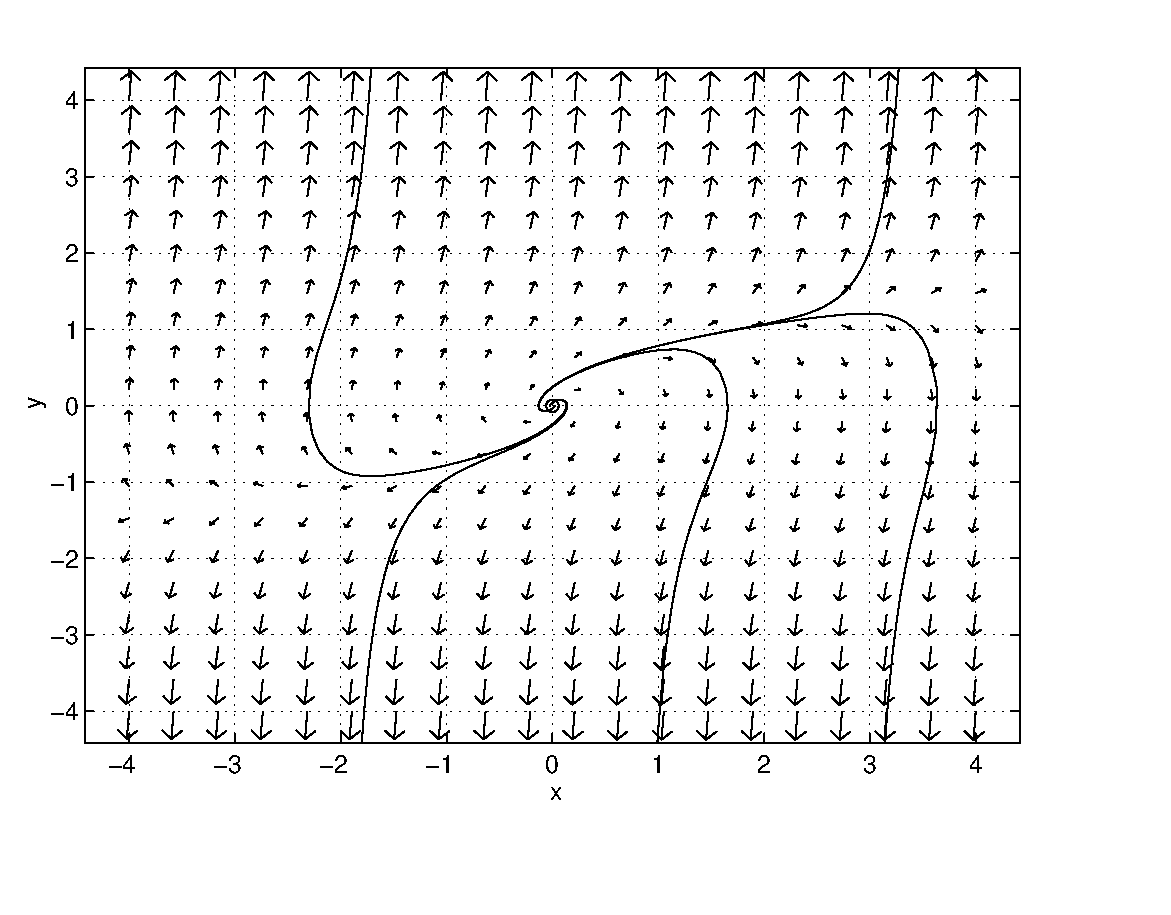
\psfig{file=exfigure/uHopfb.eps,width=2.75in}}
                \exercaptwo{e:uHopf}
\end{figure}

\exer{c9.7.5} \soln
(a) The differential equation \Ref{e:homo} is:
\[
\begin{array}{rcl}
\dot{x} & = &  y \\
\dot{y} & = &  -\rho + y + x^2 + xy
\end{array}
\]
Solve the system for $\dot{x} = 0 = \dot{y}$ to find that the equilibria
occur at $y = 0$ and $x^2 = \rho$, which is $(\pm\sqrt{\rho},0)$
for $\rho > 0$.

(b)  The Jacobian matrix of these equations is:
\[
J_{(x,y)} = \cmattwo{0}{1}{2x+y}{1+x}.
\]
At the equilibria $(\pm\sqrt{\rho},0)$ the Jacobians are
\[
J_{(\sqrt{\rho},0)}= \cmattwo{0}{1}{2\sqrt{\rho}}{1+\sqrt{\rho}} 
\AND
J_{(-\sqrt{\rho},0)}= \cmattwo{0}{1}{-2\sqrt{\rho}}{1-\sqrt{\rho}}
\]
The first Jacobian has determinant equal to $-2\sqrt{\rho}<0$; so the
first equilibrium is always a saddle.  The second Jacobian has determinant
equal to $2\sqrt{\rho}>0$ and trace equal to $1-\sqrt{\rho}$.  Since the
trace is negative when $\rho>1$, the second equilibrium is a sink.  The
discriminant of the second Jacobian is 
\[
(1-\sqrt{\rho})^2-8\sqrt{\rho}=1-10\sqrt{\rho}+\rho.
\]
The second equilibrium is a spiral when the discriminant is negative, which
it is when $1<\rho<97$.

(c)  Figures~\ref{c9.7.5}a and \ref{c9.7.5}b show that a homoclinic 
bifurcation has occurred between parameter values $\rho=1.7$ (a) and 
$\rho=1.8$ (b) with its characteristic loss of a limit cycle. 

\begin{figure}[htb]
                       \centerline{%
                       \psfig{file=exfigure/9-7-5a.eps,width=2.75in}
                       \psfig{file=exfigure/9-7-5b.eps,width=2.75in}}
                \exercaptwo{c9.7.5}
\end{figure}

\exer{c9.4.3b}
There is a homoclinic bifurcation at $\mu \approx -0.1$.  To show this,
compare Figure~\ref{c9.4.3b}b with Figure~\ref{c9.4.3b}c, which shows the
system with $\mu = -0.15$.  At $\mu = -0.15$, there is no longer a periodic
solution around the origin.  The bifurcation point occurs when the stable
and unstable orbits of the saddle point in the first quadrant coincide.

\begin{figure}[htb]
                       \centerline{%
                       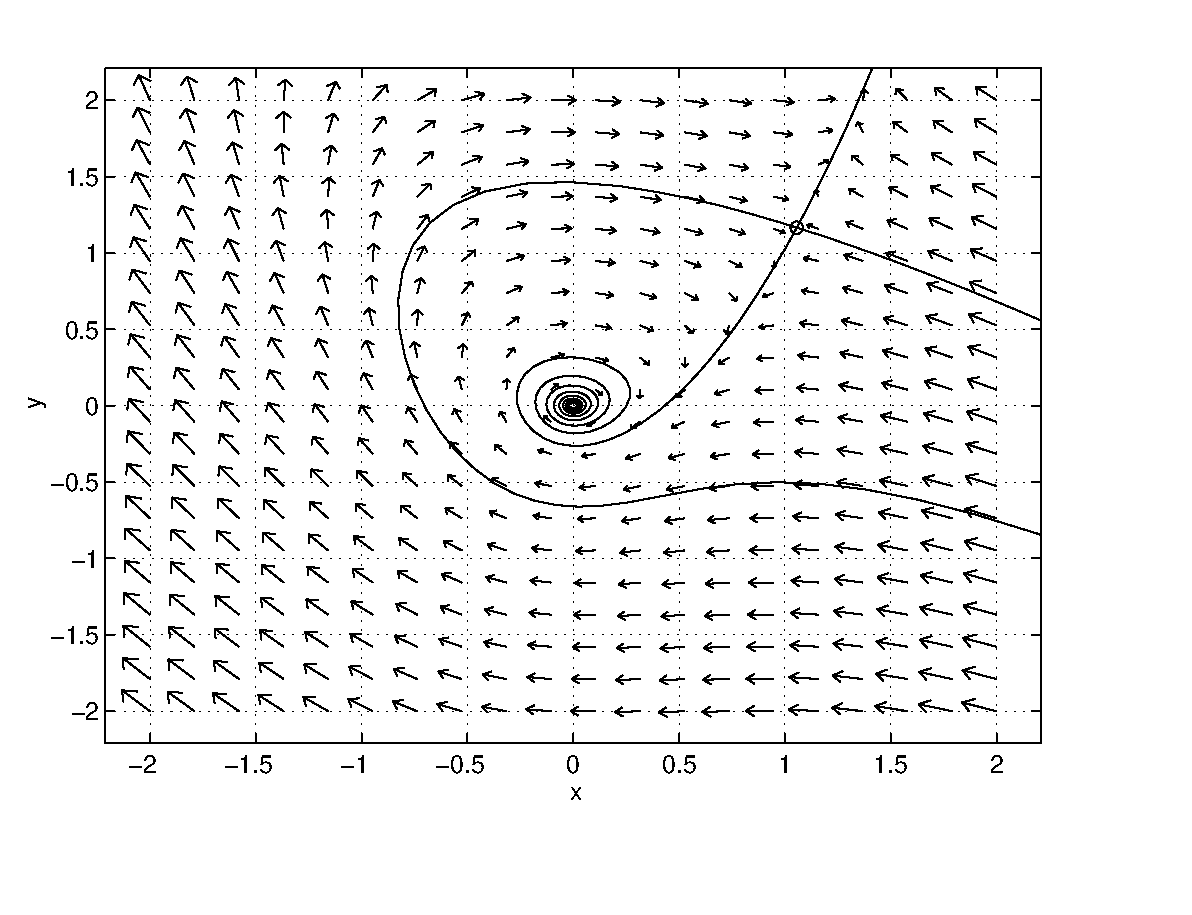
\psfig{file=exfigure/9-4-3a.eps,width=1.8in}
                       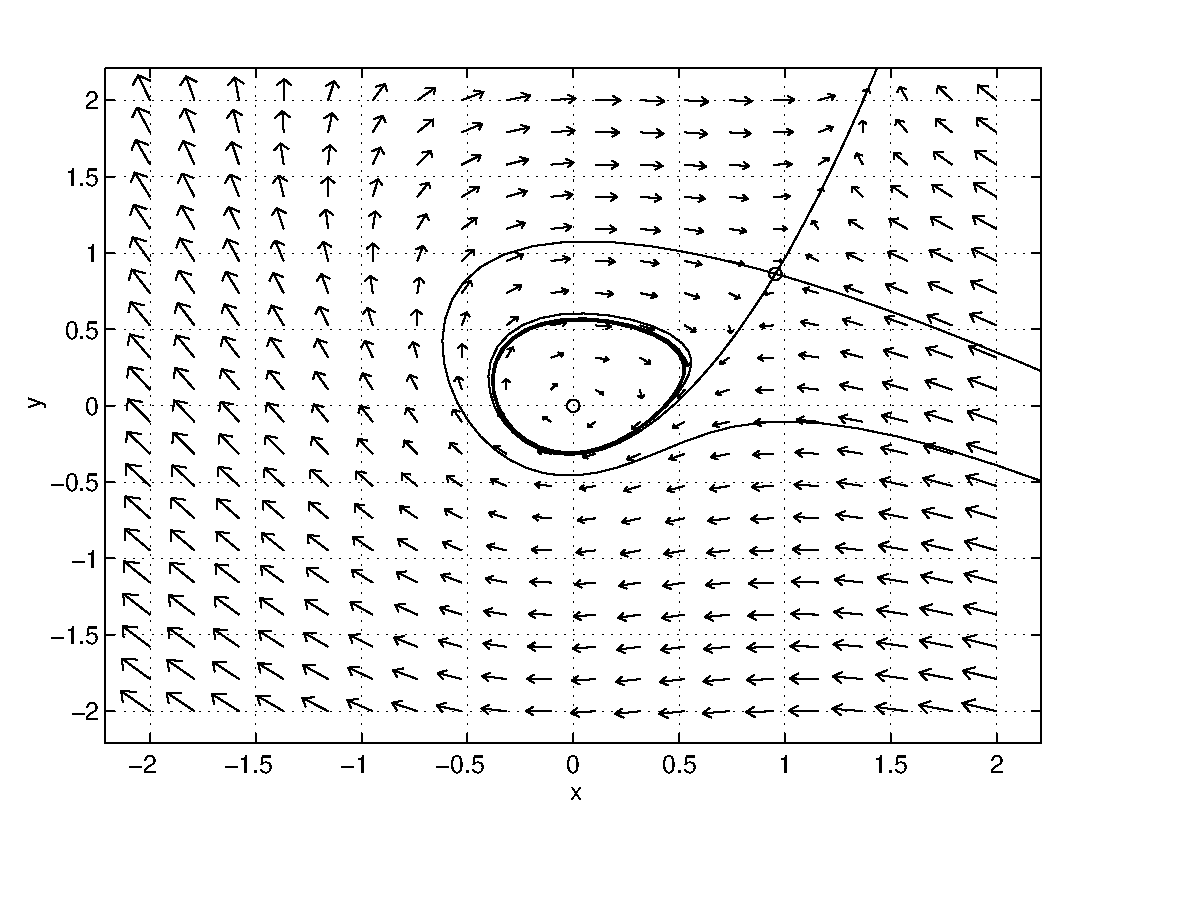
\psfig{file=exfigure/9-4-3b.eps,width=1.8in}
                       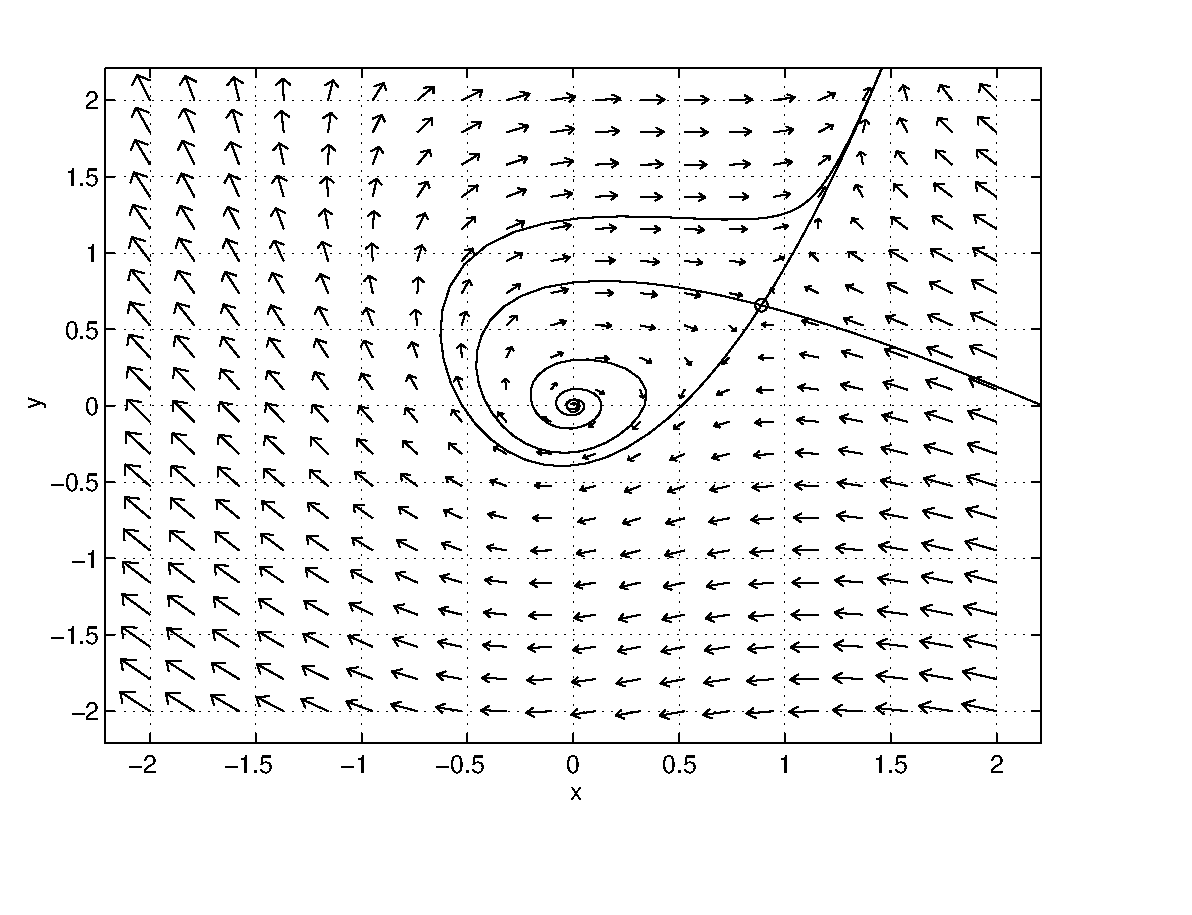
\psfig{file=exfigure/9-4-3c.eps,width=1.8in}}
		\centerline{$\mu > 0$\hspace{1.2in}$-0.1 < \mu < 0$
\hspace{1.2in}$\mu < -0.1$}
		\exercapthree{c9.4.3b}
\end{figure}

\exer{c9.4.4}
\ans The system has small amplitude periodic solutions when $\rho > 0$.

\soln Load the system into \Matlab, and graph the
system for small positive and negative values of $\rho$.



\subsection*{Section~\protect{\ref{S:CSTR}} The Continuous Flow Stirred Tank
Reactor}
\rhead{S:CSTR}{THE CONTINUOUS FLOW STIRRED TANK REACTOR}

\exer{E:CSTR5}
The system is shown in Figure~\ref{E:CSTR5}a with $\rho = 0.5$, and in
Figure~\ref{E:CSTR5}b with $\rho = 0.505$.  Note that, due to rounding
error, {\tt pplane5} may calculate the middle temperature equilibrium of
the first system as a saddle rather than a saddle node.  

\begin{figure}[htb]
                       \centerline{%
                       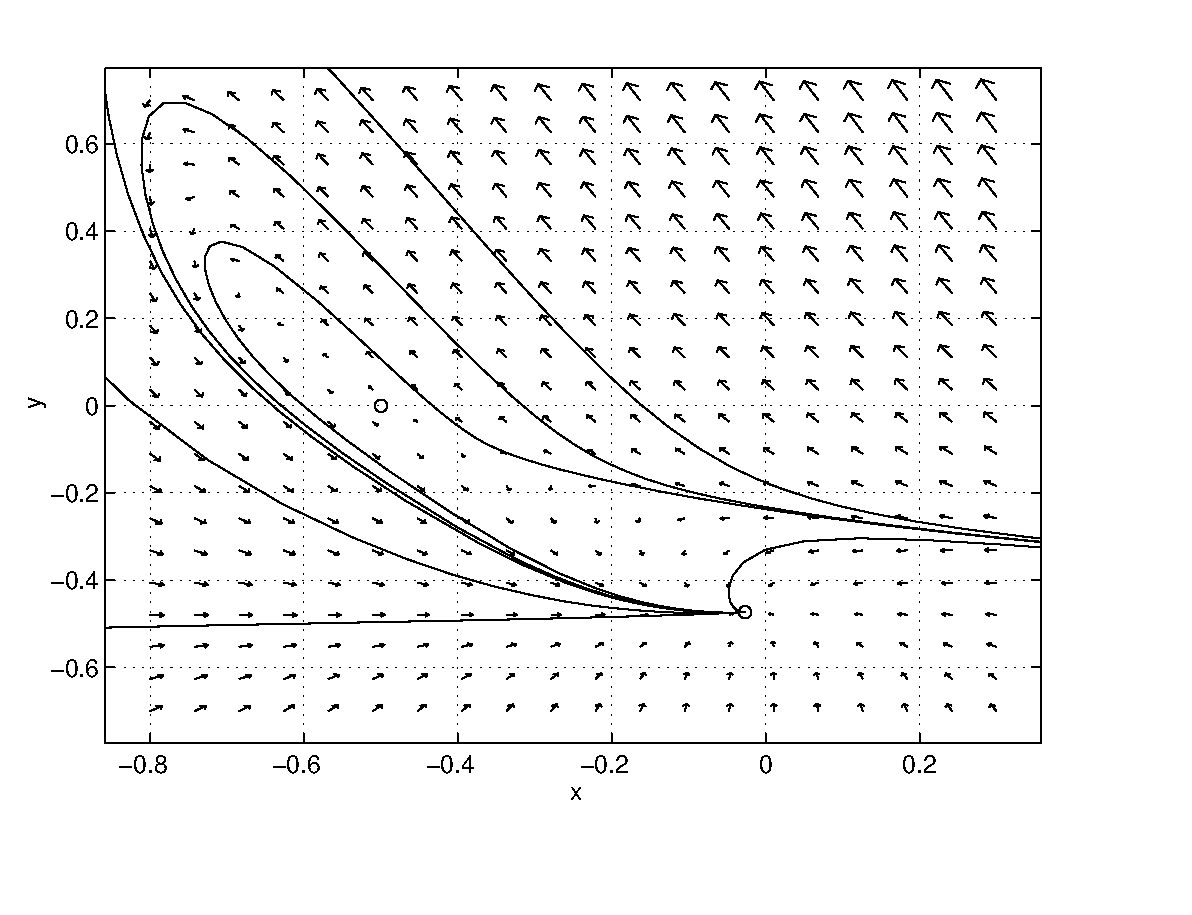
\psfig{file=exfigure/CSTR5a.eps,width=2.75in}
                       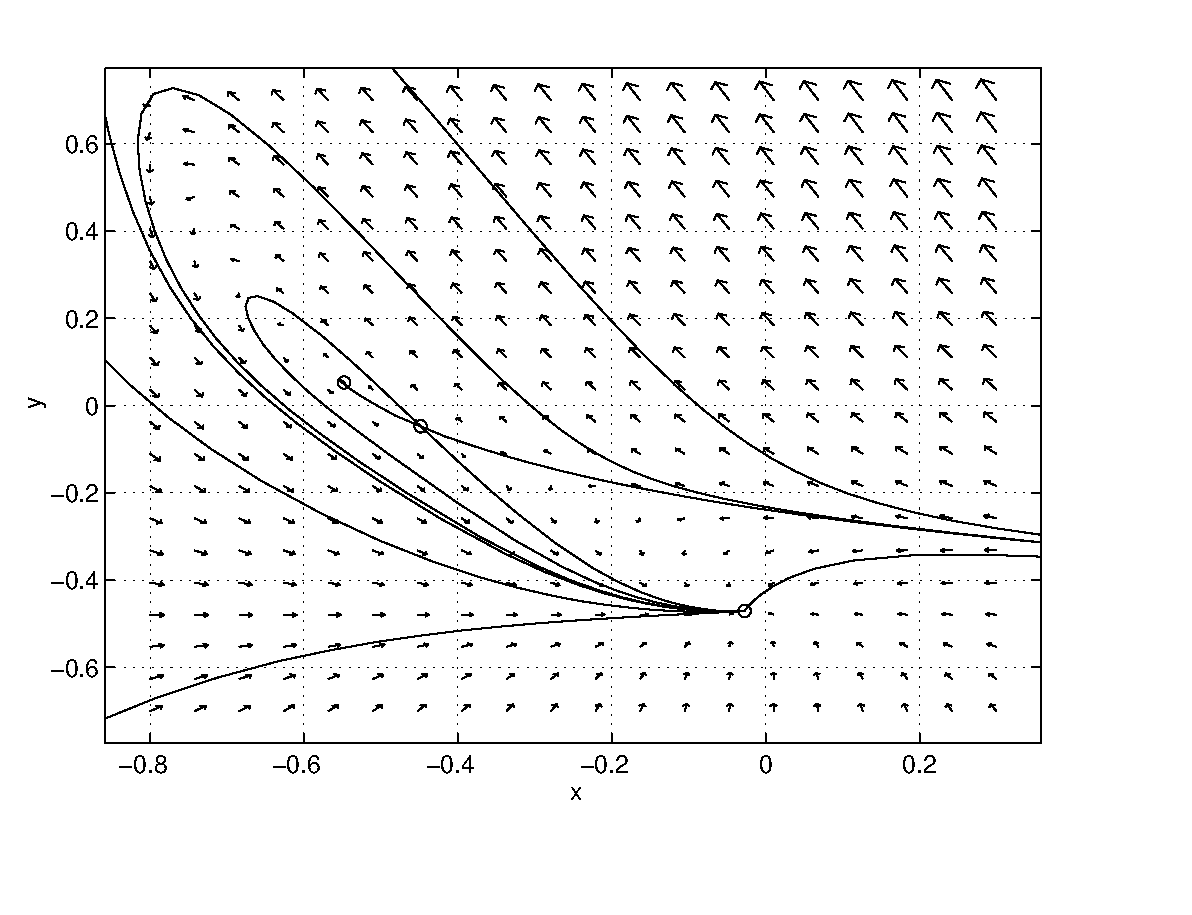
\psfig{file=exfigure/CSTR5b.eps,width=2.75in}}
                \exercaptwo{E:CSTR5}
\end{figure}



\subsection*{Section~\protect{\ref{S:GlobalBif}} The Remaining Global Bifurcations}
\rhead{S:GlobalBif}{THE REMAINING GLOBAL BIFURCATIONS}

\exer{c9.5.1}
The system has a saddle-node bifurcation of periodic solutions
at $\rho \approx 0.995$.  Figure~\ref{c9.5.1}a shows the system
with $\rho = 0.7$, at which point there are two limit cycles. 
Figure~\ref{c9.5.1}b shows the system with $\rho = 0.995$, near the point
of collision.  Figure~\ref{c9.5.1}c shows the system with $\rho = 1.1$, where
there are no periodic solutions.

\begin{figure}[htb]
                       \centerline{%
                       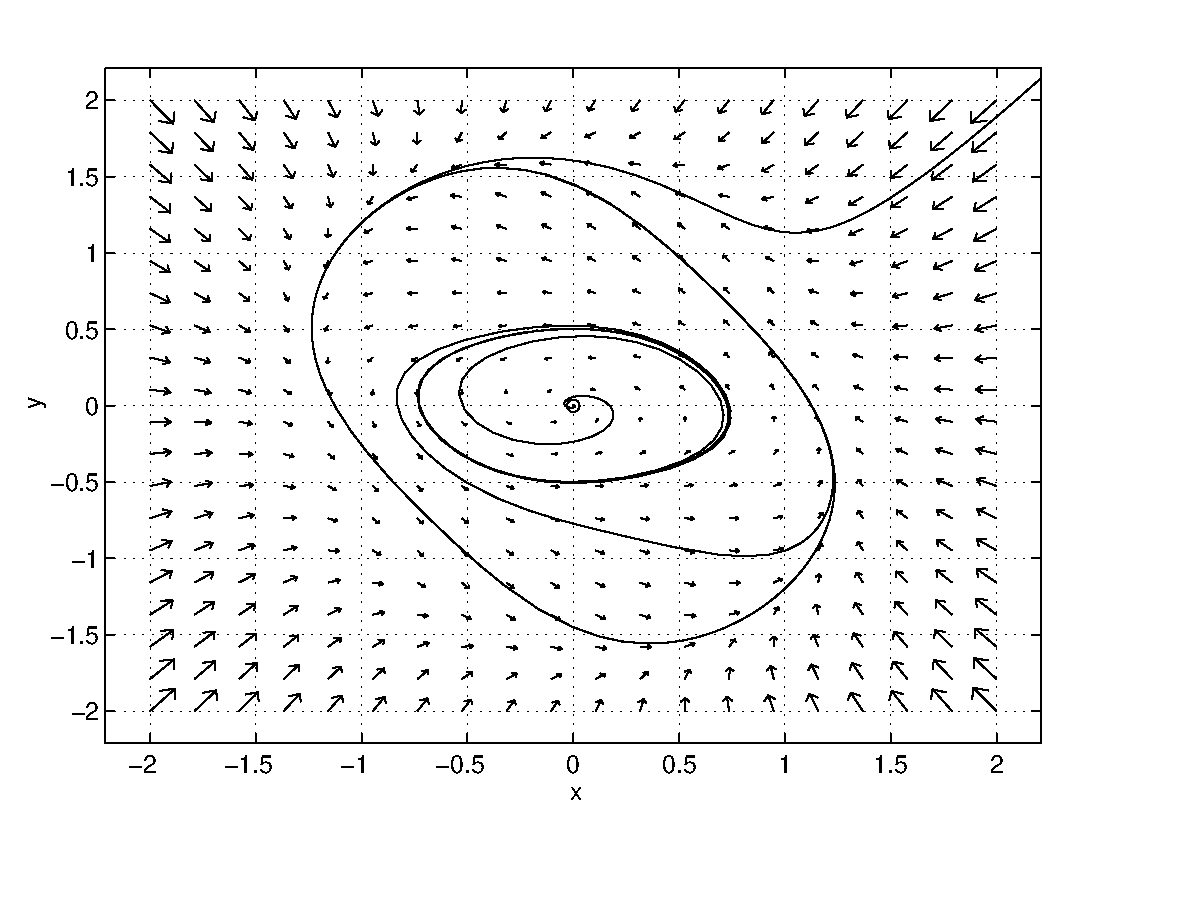
\psfig{file=exfigure/9-5-1a.eps,width=1.8in}
                       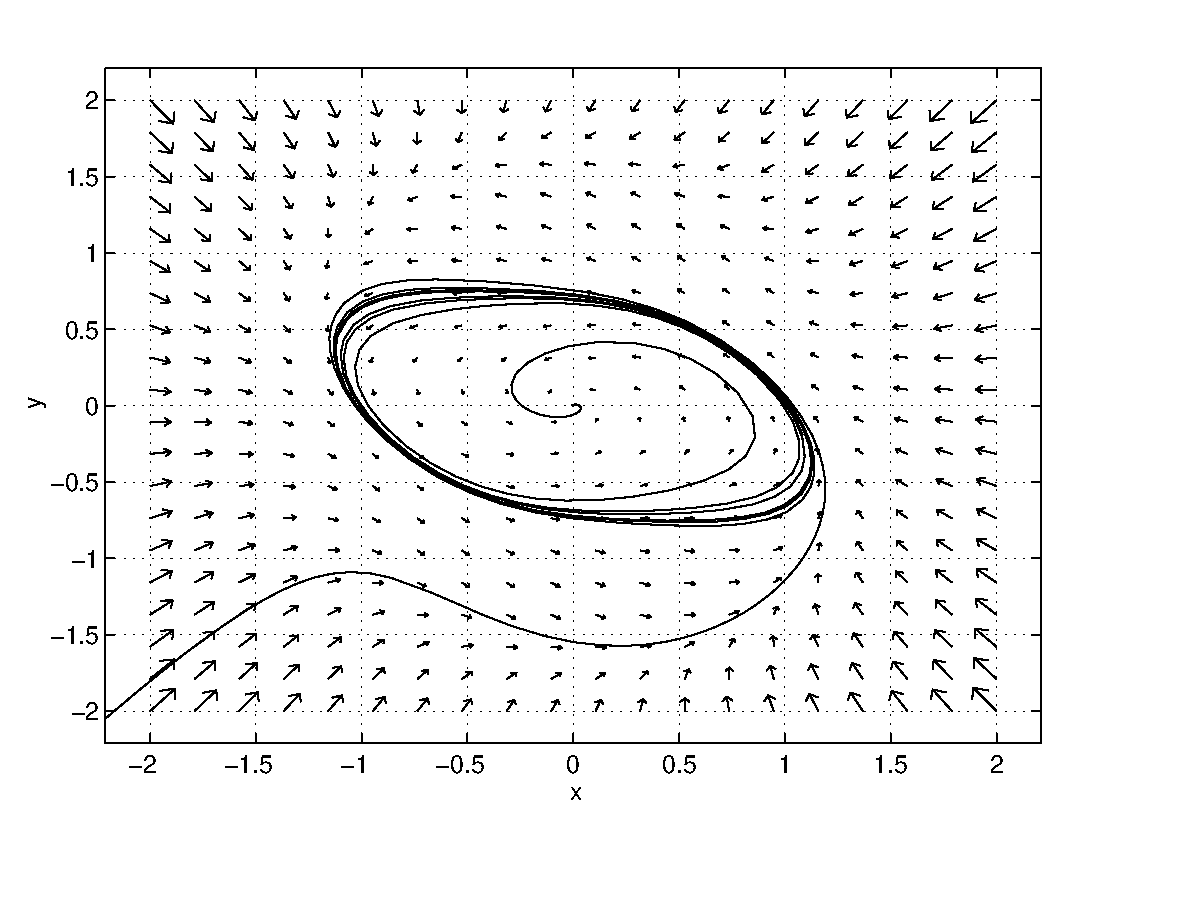
\psfig{file=exfigure/9-5-1b.eps,width=1.8in}
                       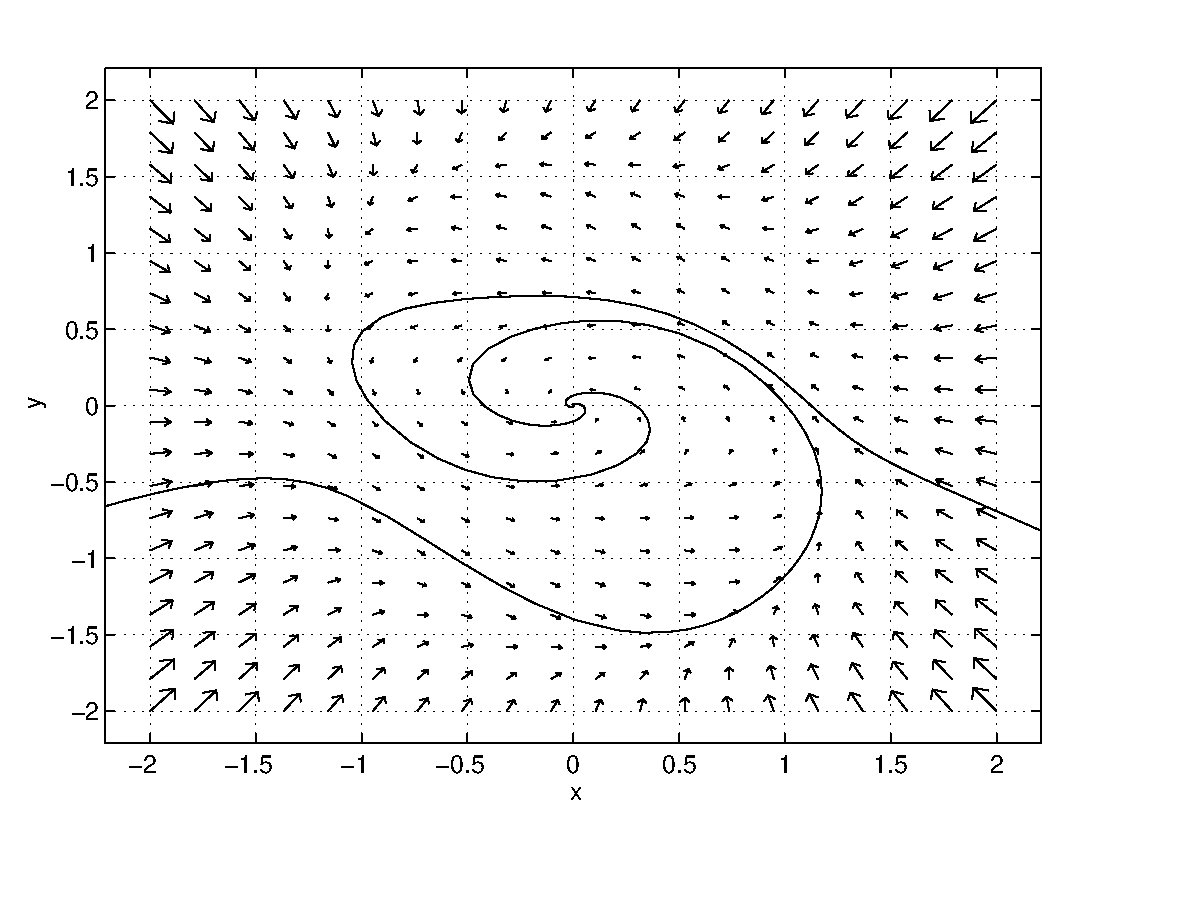
\psfig{file=exfigure/9-5-1c.eps,width=1.8in}}
		\centerline{$\rho = 0.7$\hspace{1.3in}$\rho = 0.995$
\hspace{1.3in}$\rho = 1.1$}
                \exercapthree{c9.5.1}
\end{figure}

\newpage
\exer{c9.6.2b} Figure~\ref{c9.6.2b} shows the system with $\rho = -0.03$. 
At this point, there is no periodic solution around the origin.

\begin{figure}[htb]
                       \centerline{%
                       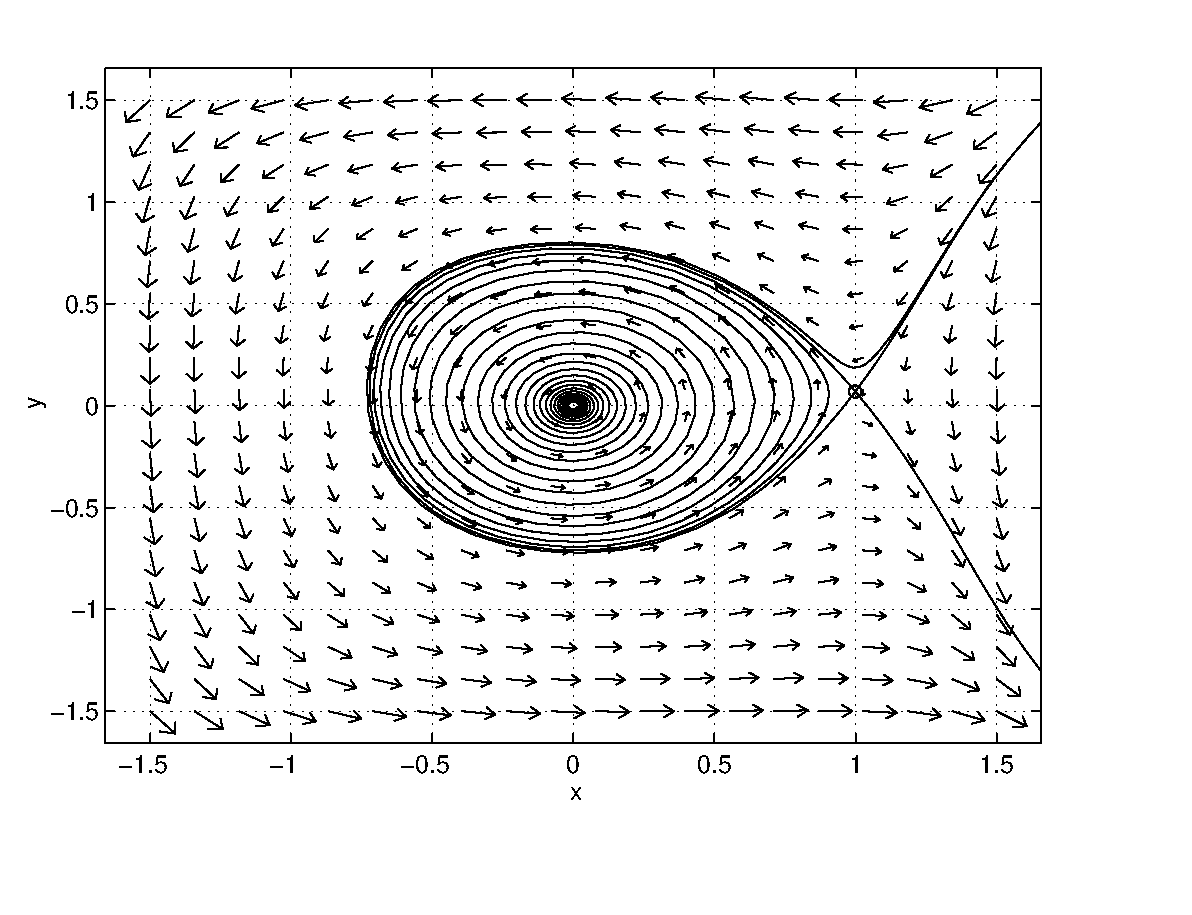
\psfig{file=exfigure/9-6-2b.eps,width=2.75in}}
		\exercap{c9.6.2b}
\end{figure}

\exer{c9.6.3a}
\ans The system appears to have an infinite number of limit cycles
as the size of the computation area increases.

\soln In the region $-2 \leq x,y \leq 2$, the system appears to have no
limit cycles.  However, in the region $-10 \leq x,y \leq 10$, there are
four limit cycles, and there are more in the larger region $-40 \leq x,y
\leq 40$.  Figure~\ref{c9.6.3a} shows the system with $\rho = 0$ on the
square $-10 \leq x,y \leq 10$.

\begin{figure}[htb]
                       \centerline{%
                       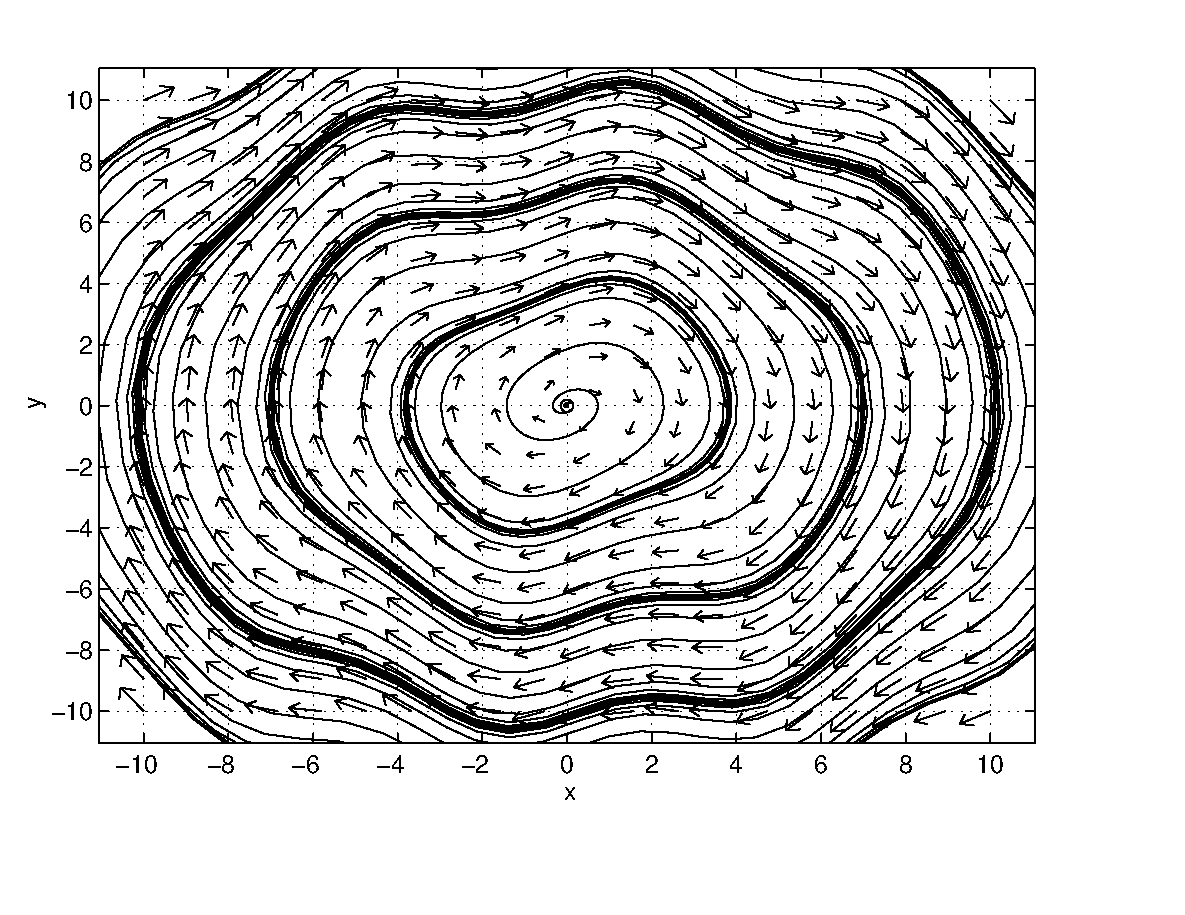
\psfig{file=exfigure/9-6-3a.eps,width=3.0in}}
		\exercap{c9.6.3a}
\end{figure}

\exer{c9.6.4a}
\ans The system has a saddle at $(x,y) \approx (0.4,-1.2)$, and a 
spiral source at $(x,y) \approx (2.0,1.9)$.

\soln Either determine the equilibria numerically from the {\tt pplane5}
graph of the system (Figure~\ref{c9.6.4a}), or compute analytically.  To
do this, solve $\dot{y} = 0$ to find that $y = x^3 - 3x$ at all equilibria.
Then, substitute this value for $y$ into $\dot{x}$ and solve $\dot{x} = 0$
to obtain $0 = x^3 + x^2 - 7.4x + 2.89$.  Find the roots of this equation
to confirm that $(x,y) \approx (0.4,-1.2)$ and $(x,y) \approx (2.0,1.9)$
are equilibria.  There is a third equilibrium at $(x,y) \approx
(-3.4,-29)$ which is not in the graph range.

\para The general Jacobian for the system is
\[
J = \cmattwo{-1 + 2(x - \rho)}{1}{-3x^2 + 3}{1}.
\]
Thus, when $\rho = 1.7$, $\trace(J) = 2(x - 1.7)$ and
$\det(J) = 3x^2 + 2(x - 1.7) - 4$.  At $(x,y) \approx (0.4,-1.2)$,
$\det(J) \approx -6.1 < 0$, so the equilibrium is a saddle.  At
$(x,y) \approx (2.0,1.9)$, $\det(J) \approx 8.6 > 0$, $\trace(J) \approx
0.6 > 0$, and $D = (\trace(J))^2 - t\det(J) \approx -34 < 0$.  Therefore,
this equilibrium is a spiral source.

\exer{c9.6.4c} A Hopf bifurcation occurs between $\rho = 1.85$
(Figure~\ref{c9.6.4c}a) and $\rho = 2.1$ (Figure~\ref{c9.6.4c}b).  The
spiral source passes through a center and becomes a
spiral sink.  At this point, the periodic solution disappears.

\begin{figure}[htb]
                       \centerline{%
                       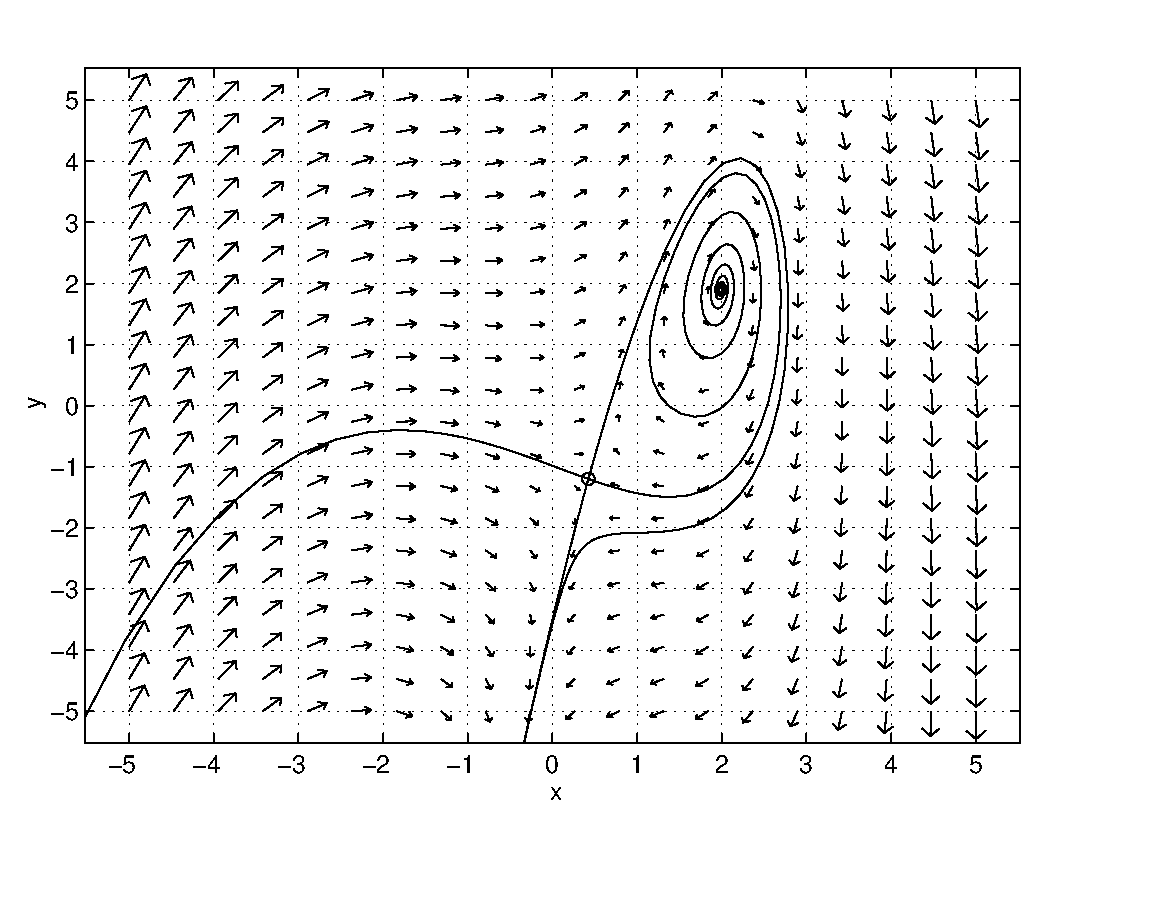
\psfig{file=exfigure/9-6-4a.eps,width=1.8in}
                       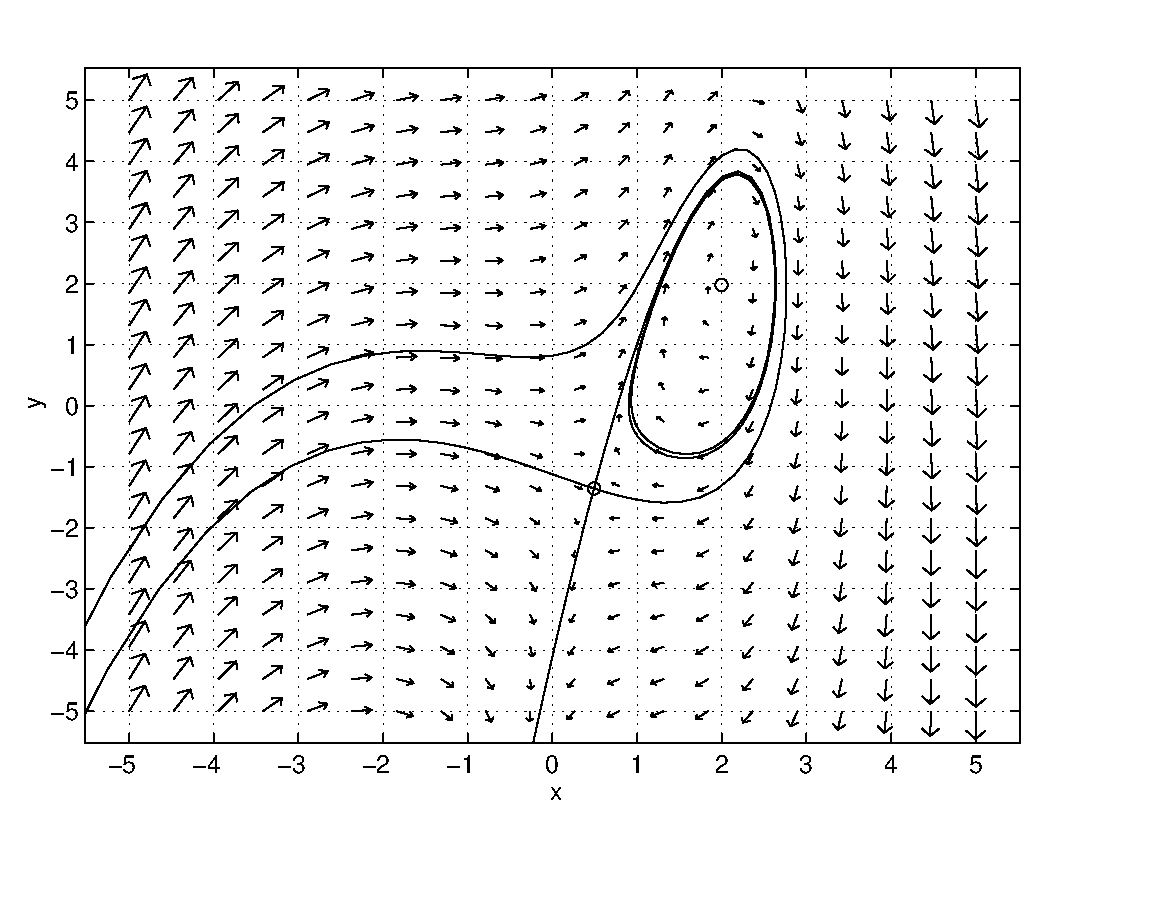
\psfig{file=exfigure/9-6-4b.eps,width=1.8in}
                       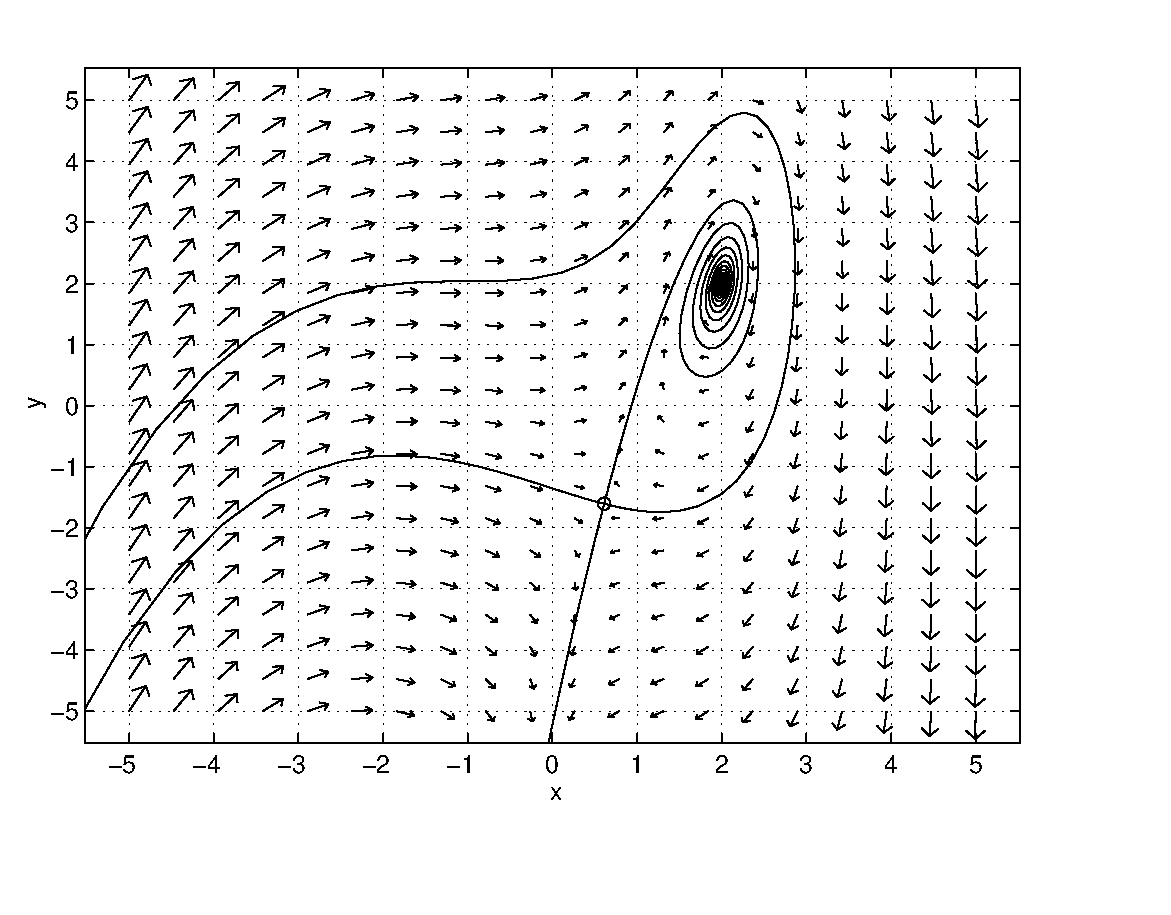
\psfig{file=exfigure/9-6-4c.eps,width=1.8in}}
	\centerline{$\rho = 1.7$\hspace{1.3in}$\rho = 1.85$\hspace{1.3in}
$\rho = 2.1$}
	\centerline{Figure~\ref{c9.6.4a}\hspace{1.2in}Figure~\ref{c9.6.4c}a
\hspace{1.2in}Figure~\ref{c9.6.4c}b}
\end{figure}

\exer{c9.6.5a}
\ans For any values of $\rho$, the system has saddle points at
\[
(x,y) = (-\rho + \sqrt{\rho^2 + 4},0) \AND
(x,y) = (-\rho - \sqrt{\rho^2 + 4},0)
\]
and a spiral sink at the origin.

\soln Set $\dot{x} = \dot{y} = 0$.  Then $y = 0$, and
$0 = x^3 + \rho x^2 - x$, so there are equilibria at the origin, and at
the roots of $x^2 + \rho x - x$.

\exer{c9.6.5c}
A heteroclinic bifurcation occurs at $\rho \approx 0.141$.  At this
point, an unstable orbit of the leftmost saddle point coincides with a
stable orbit of the rightmost saddle point.



\subsection*{Section~\protect{\ref{S:SNB}} Saddle-Node Bifurcations Revisited}
\rhead{S:SNB}{SADDLE-NODE BIFURCATIONS REVISITED}

\exer{c9.3.1}
(a) A steady-state bifurcation occurs on a function $f(x,\rho)$ at a
point $(x,\rho) = (x_0,\rho_0)$ if $f(x_0,\rho_0) = 0$ and
$f_x(x_0,\rho_0) = 0$.  In this case, let $(x_0,\rho_0) = (0,0)$.
Then
\[ \begin{array}{rcccl}
f_1(x_0,\rho_0) & = & \rho_0 - x_0^3 & = & 0 \\
f_{1x}(x_0,\rho_0) & = & -3x_0^2 & = & 0 \end{array}
\qquad
\begin{array}{rcccl}
f_2(x_0,\rho_0) & = & \rho_0x_0 - x_0^2 & = & 0 \\
f_{2x}(x_0,\rho_0) & = & \rho_0 - 2x_0 & = & 0. \end{array}
\]
Therefore, $f_1$ and $f_2$ have steady-state bifurcations at $(x,\rho)
= (0,0)$.

(b) A saddle-node bifurcation occurs on a function $f(x,\rho)$ at a point
$(x,\rho) = (x_0,\rho_0)$ if $f$ has a steady-state bifurcation at this
point, and if $f_\rho(x_0,\rho_0) \neq 0$ and $f_{xx}(x_0,\rho_0) \neq 0$.
Let $(x_0,\rho_0) = (0,0)$.  Then
\[
f_{1xx}(x_0,\rho_0) = -6x = 0 \AND
f_{2p}(x_0,\rho_0) = x = 0,
\]
so neither $f_1$ nor $f_2$ has a saddle-node bifurcation at $x = 0$.

(c) The bifurcation diagram for $f_1$ is shown in Figure~\ref{c9.3.1}a, and
the diagram for $f_2$ is shown in Figure~\ref{c9.3.1}b.  Saddle-node
bifurcations occur only when equilibria appear or disappear.
Figure~\ref{c9.3.1}a shows that $f_1$ has one equilibrium for all $\rho$,
and Figure~\ref{c9.3.1}b shows that $f_2$ has two equilibria for all
$\rho$.  Thus, neither function has a saddle-node bifurcation at the origin.

\begin{figure}[htb]
                       \centerline{%
                       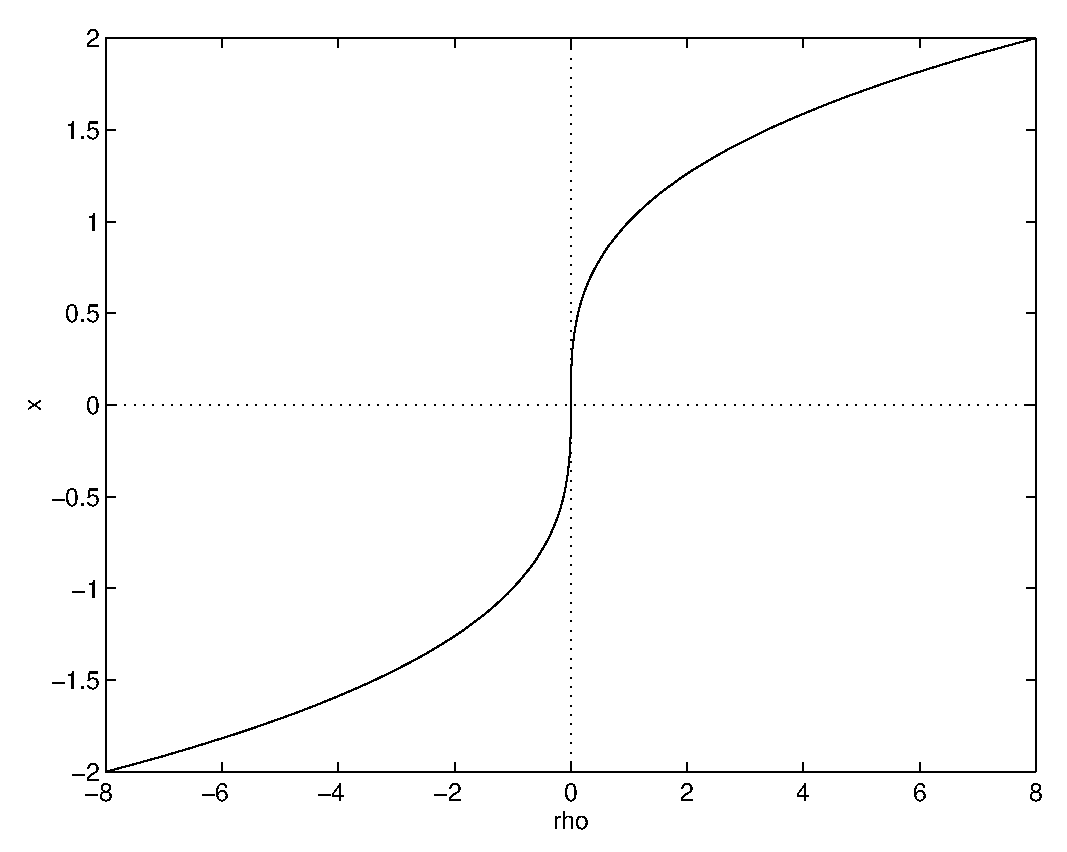
\psfig{file=exfigure/9-3-1a.eps,width=2.75in}
                       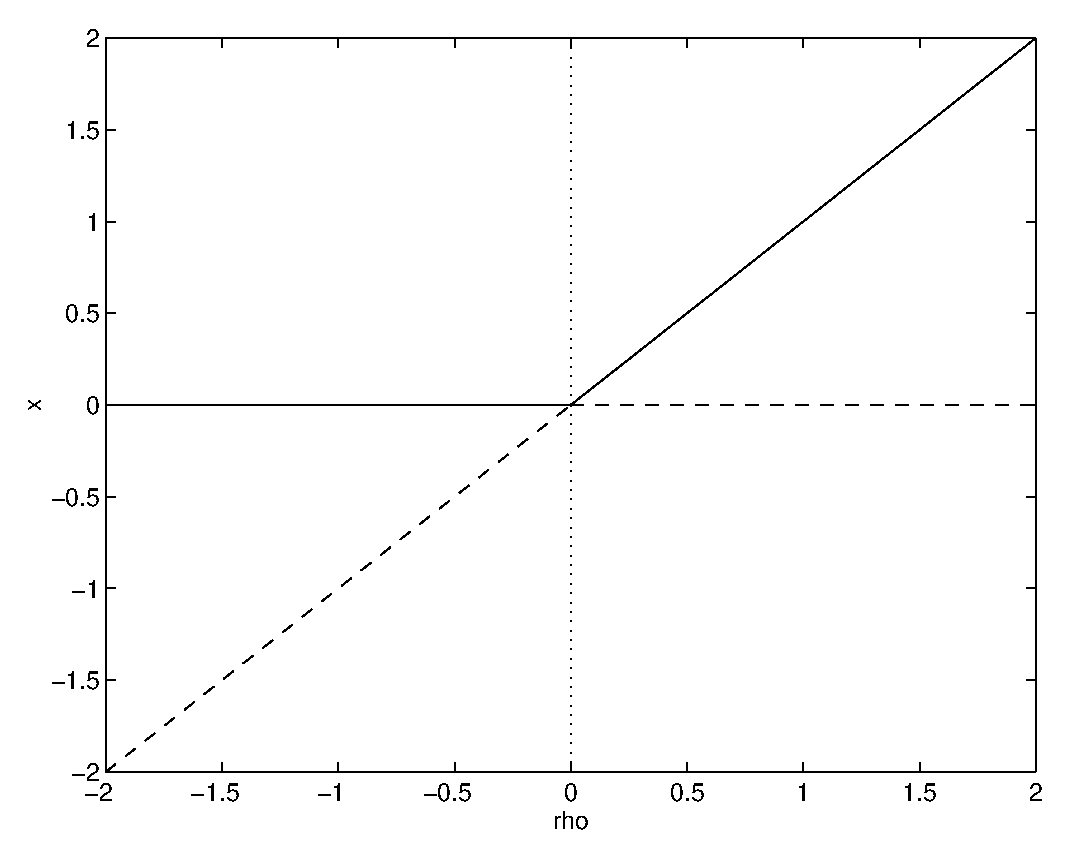
\psfig{file=exfigure/9-3-1b.eps,width=2.75in}}
                \exercaptwo{c9.3.1}
\end{figure}

\exer{c9.3.2}
\ans There are two equilibria near $x = 3$ when $\rho > 1$.

\soln Calculate
\[
f(3,1) = 0, \quad
f_x(3,1) = 0, \quad
f_\rho(3,1) = -6 \neq 0, \AND
f_{xx}(3,1) = 16 \neq 0.
\]
Therefore, $f$ has a saddle-node bifurcation at $x = 3$ when $\rho =
1$.  Note that Theorem~\ref{T:saddlenode} states
that if $a < 0$, then there are two equilibria near $x_0$ for $\rho >
\rho_0$.  In this case,
\[
a = \frac{f_{xx}(x_0,\rho_0)}{f_p(x_0,\rho_0)} = -\frac{8}{3} < 0.
\]

\exer{c9.3.4}
To show that the origin is a bifurcation point of $F$ when $\rho = 0$, we
must show the following:

(a) $F(0,0) = 0$.

(b) Let $J = dF_{(0,0)}$.  Then $\det(J) = 0$ and $\trace(J) \neq 0$.

(c) There exist nonzero vectors $v$ and $w$ such that $Jv = 0$ and
$J^tw = 0$.

\soln Let
\[
\vectwo{g(X,\rho)}{h(X,\rho)} = F(X,\rho) = 
\cvectwo{\rho q_1 + x + \alpha x^2 + \beta xy + \gamma y^2}
{\rho q_2 + \delta x^2 + \epsilon xy + \varphi y^2}.
\]

(a) Indeed, $g(0,0) = 0 = h(0,0)$, so $F(0,0)$ is an equilibrium point.

(b) Find the Jacobian
\[
J = \left.\cmattwo{1 + 2\alpha x + \beta y}{\beta x + 2\gamma y}
{2\delta x + \epsilon y}{\epsilon x + 2\varphi y}\right|_{(0,0)} =
\mattwo{1}{0}{0}{0}.
\]
Since $\det(J) = 0$ and $\trace(J) = 1 \neq 0$, there
is a bifurcation point at the origin with $\rho = 0$.

(c)  To verify that the nondegeneracy conditions are satisfied, find $v$
and $w$.  In this case $v = w = (0,1)^t$.  Then verify
\[
w \cdot F_\rho(X_0,\rho_0) = \vectwo{0}{1} \cdot \vectwo{q_1}{q_2}
= q_2.
\]
So, condition \Ref{e:2deig} is satisfied when $q_2 \neq 0$.  To
verify \Ref{e:2dbifur}, compute the vector
\[
F_0 = 0\vectwo{g_{xx}}{h_{xx}} + 0\vectwo{g_{xy}}{h_{xy}} +
\vectwo{g_{yy}}{h_{yy}} = \vectwo{2\gamma}{2\varphi}
\]
and calculate
\[
w \cdot F_0 = \vectwo{0}{1} \cdot \vectwo{2\gamma}{2\varphi}
= 2\varphi.
\]
So, the origin is a saddle node of $F$ with $\rho = 0$ when
$q_2 \neq 0$ and $\varphi \neq 0$.



\subsection*{Section~\protect{\ref{S:HopfBif}} *Hopf Bifurcations Revisited}
\rhead{S:HopfBif}{*HOPF BIFURCATIONS REVISITED}

\exer{c9.6.1a}
\ans The only equilibria of this system occur at the origin and a point of
Hopf bifurcation occurs at $\rho=0$.  The eigenvalue crossing condition is
satisfied.

\soln  To find the equilibria solve $\dot{y}=0$ for $x=0$ and $\dot{x}=0$ for
$y=0$.  The Jacobian matrix at the origin is 
\[
J(\rho) = \mattwo{\rho}{-1}{1}{0}.
\]
Thus, $\trace(J(\rho))=0$ only when $\rho=0$.  So a Hopf bifurcation point
can only occur at $\rho=0$.  Finally, note that 
\[
\frac{d}{dt}\trace(J(\rho)) = 1 \neq 0;
\]
So the eigenvalue crossing condition is satisfied.



\end{document}
